\subsection{OracleVM}

Este software tem com principal funcionalidade, a gestão do sistema de virtualização através
de uma plataforma web que pode ser acedida atráves do seguinte endereço\\
\emph{https://<IP\_DO\_SERVIDOR>:4443/OVS}, figura~\ref{fig:ovm1}.

\begin{figure}[H]
    \begin{center}
        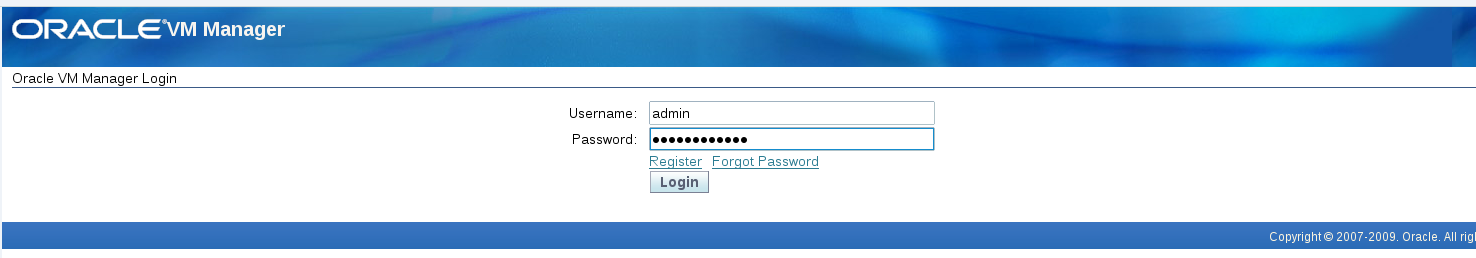
\includegraphics[width=15cm]{include/img/ovm1.png}
    \end{center}
    \caption{Login OracleVM Manager}
    \label{fig:ovm1}
\end{figure}

Esta ferramenta permite a gestão dos servidores reais que suportam o sistema de virtualização,
figura~\ref{fig:ovm2}, bem como a gestão das respectivas máquinas virtuais que irão fazer
parte da infra-estrutura virtual,figura~\ref{fig:ovm3}.

\begin{figure}[H]
    \begin{center}
        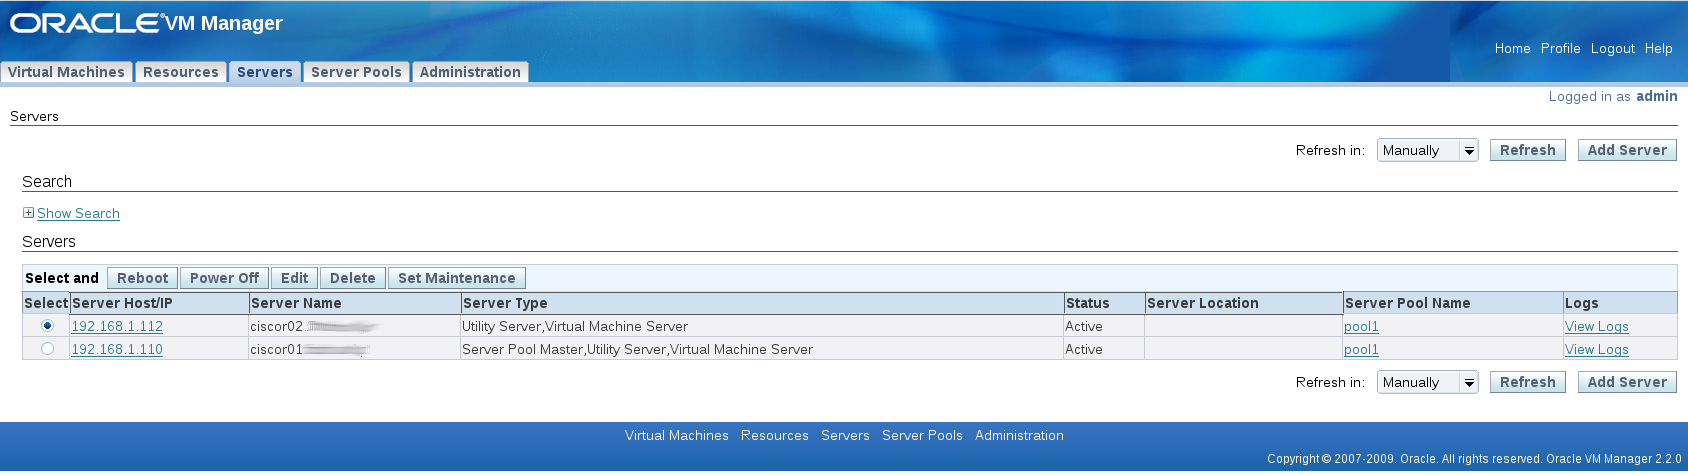
\includegraphics[width=15cm]{include/img/ovm2.png}
    \end{center}
    \caption{Máquinas Reais OracleVM Manager}
    \label{fig:ovm2}
\end{figure}



\begin{figure}[H]
    \begin{center}
        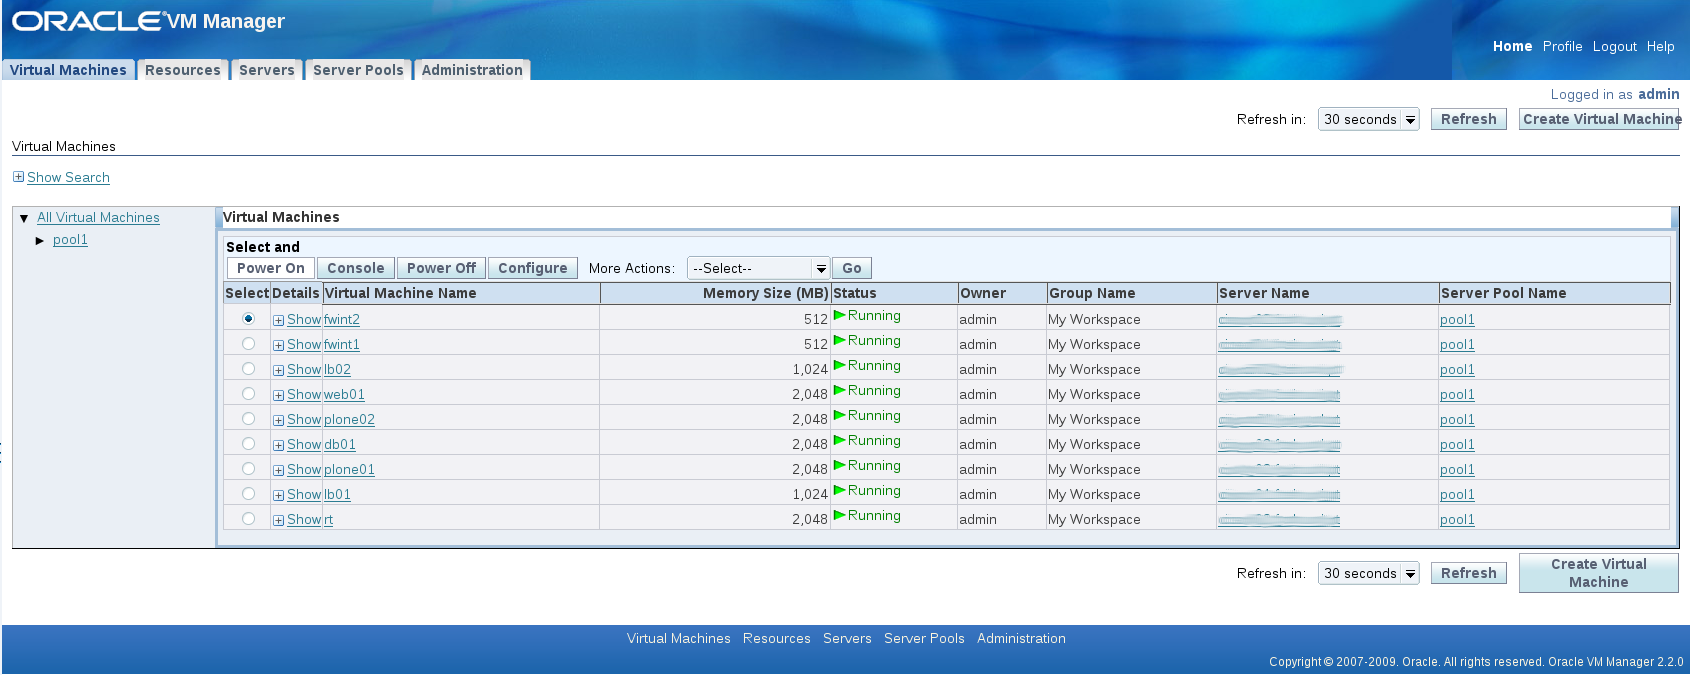
\includegraphics[width=15cm]{include/img/ovm3.png}
    \end{center}
    \caption{Máquinas Virtuais OracleVM Manager}
    \label{fig:ovm3}
\end{figure}

Para mais informações acerca do OracleVM Manager, podem aceder ao link do manual que é disponibilizado pela
Oracle(\emph{\url{http://download.oracle.com/docs/cd/E15458\_01/doc.22/e15441/toc.htm}}).
